\subsection{Linear Regression}

% TODO: Cite sources:
% - https://www.kaggle.com/c/house-prices-advanced-regression-techniques/data


% TODO: Explain this better. It sounds robotic and unintuitive. This shit needs
% to be a STORY
The main focus of this section is predicting a real number when given a set of
other numbers, or using pre-recorded inputs and outputs to generate new outputs
for any input we may need. In a linear sense, we are finding a continuous
function that takes in one number and spits out another using previously
gathered data. So the question is, how do we form this function?


\begin{figure}[t!]
\centering
    \begin{tikzpicture}
        \selectcolormodel{gray}
        \begin{axis}[
                title = {HOUSE PRICES AND WITH PLOT AREAS},  % whatever name you want
                xlabel = {Plot Area in 1,000 ft$^2$},
                ylabel = {House Price in \$100,000},
                tick label style={/pgf/number format/fixed},
                scaled y ticks = false,
                scaled x ticks = false,
                yticklabel={
                    \fpeval{\tick / 100000}               % Divide the y coordinate/1000
                },
                xticklabel={
                    \fpeval{\tick / 1000}               % Divide the y coordinate/1000
                },
            ]
            \addplot[
                only marks,
                select coords between index={1}{50},
                ] table[col sep=comma]{linreg_houseprice.csv};
        \end{axis}
    \end{tikzpicture}
    \caption{List of plot areas and selling prices for houses in Ames, Iowa.
    Looking at these kind of plots, we can try to find correlations in the data
    that help us predict what future houses may cost in that market.}
    \label{fig:hp}
\end{figure}

Let's look at the scatterplot in Figure \ref{fig:hp}, which shows a bit of
housing data from Ames, Iowa. When observing it, our goal is to create a model
that will take a plot area and give us a house price that best fits the examples
recorded. So we start by asking, what kind of representation of data best aligns
with what we are asking? How can we find patterns in this data to predict what
price might be associated to a specified plot area? How can we do this
autonomously?

First, we can identify that there is a positive correlation when comparing each
plot area with its corresponding price, showing us that as plot area increases,
so does the house price. There are some outliers for this case, but generally
this trend is consistent. Additionally, we can take note that there is some
base price for every house in the area. We can observe this with the fact that
we don't see any houses that cost a negative amount. That would just be
ridiculous and would cause an economic downturn. More intuitively, we can
observe this by the fact that the goal of selling a house is to make money, so
assuming the smallest house you could buy is around 1,000 ft$^2$, we would
never see such a house costing \$0. As such, we should be able to draw a
straight line through the data from some offset such that we get fairly close
to all of the recorded examples.

This relationship is the basis for any linear function of the form $y=ax + b$
with the slope coefficient $a$ describing the correlation between housing
price/plot area and the offset $b$ describing the overall starting price for
houses in Ames. We prescribe these coefficients to the vector of prices $\theta
= \begin{pmatrix}\theta_0 \\ \theta_1\end{pmatrix}$ such that the base price is
$b = \theta_0$ and the price per ft$^2$ of plot area is $a=\theta_1$. This
coefficient vector is known as the \emph{weight vector} since we adjust the
values in $\theta$ until we find coefficients that best fit the data. In
context, this linear function will predict the ideal price of any house in
Ames after learning from the experiences we feed it.

Examining these properties sets us up to form a hypothesis for how house prices
are determined. Let $X$ be the training set, i.e. the set containing all of the
recorded plot areas. Let $X^{(i)}$ be the plot area for the $i$th feature in
$X$. From what we've discussed, the equation
\begin{equation}
    hypothesis_{\theta}(X^{(i)}) = \theta_0 + \theta_1X^{(i)}
\end{equation}
should ideally give us the correct price for $X^{(i)}$. The key word in the last
sentence is \emph{ideally} since the hypothesis function will only give us 100\%
accuracy when all the data in the data set lies exactly on the line formed by
the hypothesis. This would mean that each square foot of plot area would cost
the exact same amount at every house you check. However optimal this is, it is
generally not the case. Instead, we look to maximize the accuracy of this
function or otherwise minimize the \emph{loss}.


We begin measuring the error of our hypothesis by comparing it with the
previously collected data.  An intuitive way for measuring the  error of the
hypothesis would be by measuring the shortest distance between the value it
predicts and the recorded value since this, in a literal sense, tells us how far
off our prediction was from the result. This, along with other measurements,
is discussed more in \placeholder. However, we will still derive the process for
finding this distance here until that section is written.

\begin{wrapfigure}{O}{0.5\textwidth}
    \centering
    \resizebox{0.5\textwidth}{!}{
        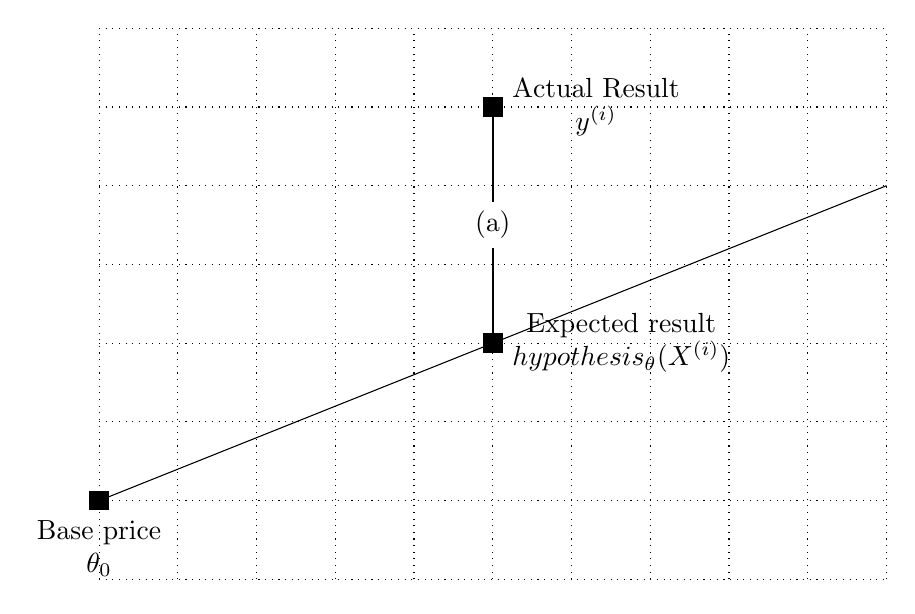
\begin{tikzpicture}[every label/.style={align=center}]
            \node[draw, fill=black, label=right:{Actual Result \\ $y^{(i)}$}] (v1) at (5,6) {};
            \node[draw, fill=black, label=right:{Expected result \\ $hypothesis_{\theta}(X^{(i)})$}] (v2) at (5,3) {};
            \node[draw, fill=black, label=below:{Base price \\ $\theta_0$}] (v3) at (0,1) {};

            \draw[dotted] (0,0) grid (10,7);
            \draw (0,1) -- (10,5);
            \draw[thick] (v1) -- (v2) node [midway, fill=white] {(a)};
        \end{tikzpicture}
    }
    \caption{Visual representation of the distance between expected and actual
    results.}
    \label{fg:err}
\end{wrapfigure}

We see how this is found in Figure \ref{fg:err} by examining the case for a
single feature. First, the hypothesis function predicts a result for $X^{(i)}$.
We then compare this to the original result $y^{(i)}$ by finding the distance
between these two points, also known as the \emph{residual} or the \emph{error}
and is measured by the length of the line marked by (a). We can find this
distance in two ways, those being the \emph{squared distance} and the
\emph{absolute distance}, both of which result in a positive value. We prefer
the squared distance in this scenario because the algebra comes out much neater
than that of the absolute distance, most notably in the calculations later on in
this section, however both have their pros and cons when determining residual
error. This will be further discussed in \placeholder.

The squared distance between any two points is the squared norm $\| point_1 -
point_2 \|^2$ or equivalently $(point_{1x}-point_{2x})^2$ $+$
$(point_{1y}-point_{2y})^2$. When we substitute in the points $(X^{(i)},
hypothesis_{\theta}(X^{(i)}))$ and $(X^{(i)}, y^{(i)})$, the $x$ values cancel
out, reducing this down to the distance between the two $y$ values. Putting this
all together, we define our loss function as:
\begin{equation}
    loss_{\theta}(X^{(i)}, y^{(i)}) = (hypothesis_{\theta}(X^{(i)}) - y^{(i)})^2
\end{equation}

Now that we have a method for calculating the amount of loss a single feature
has with weights $\theta$, we need a method for determining the overall loss of
our weights. That is, we need some function, called the \emph{cost function},
that quantifies the uncertainty of $\theta$. There are several such methods for
quantifiying this uncertainty, however those are discussed further in Section
\placeholder. For now, an effective method for achieving this is by averaging
the loss over the entire training set. This method is known as the \emph{mean
squared error (MSE)}. So if we let $m$ be the number of features in $X$, the
cost function
\begin{subequations}
    \begin{align}
        cost(\theta) = \frac{1}{m}\sum_{i=1}^m loss_{\theta}(X^{(i)}, y^{(i)}) \\
    \intertext{will give us a good estimate for how well $\theta$ is performing
        in the hypothesis. Expanded out, this is equivelent to}
        cost(\theta) = \frac{1}{m}\sum_{i=1}^m (\theta_0 + \theta_1X^{(i)} -
        y^{(i)})^2
    \end{align}
\end{subequations}
.

Since we have this function that measures the overall loss, the next step would
be finding values of $\theta$ that minimize this value. This would mean finding
a base price and price per ft$^2$ that matches the data enough such that the
hypothesized price would be reasonably close to the recorded price. What we're
essentially looking for are \emph{the coordinates of a point in the cost
function's domain that correspond to the lowest lowest possible value for the
cost}. To do this, let's consider the shape of the cost function.

\begin{figure}[t!]
    \centering
    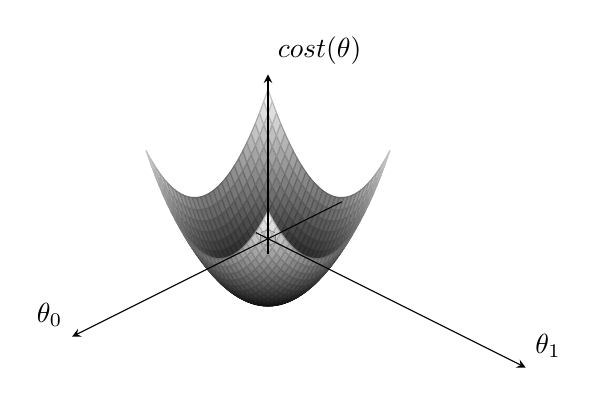
\begin{tikzpicture}[
        declare function = {
            Z(\x, \y) = ((\x-8)^2 + (\y-8)^2)/8;
        }
    ]
        \begin{axis}[
            view = {135}{30},
            colormap/blackwhite,
            axis equal,
            axis lines = center,
            axis on top,
            ticks = none,
            set layers = default
            xmin = 0, ymin = 0, zmin = 0,
            xlabel=$\theta_0$, ylabel={$\theta_1$}, zlabel={$cost(\theta)$},
            xlabel style={anchor=south east},
            ylabel style={anchor=south west},
            zlabel style={anchor=south west},
            enlargelimits,
            tick align=inside,
            domain=0:16,
            y domain = 0:16,
            samples=30,
            z buffer=sort,
            minor tick=1,
            ]
            \addplot3 [surf] {Z(x, y)};
        \end{axis}
    \end{tikzpicture}
    \caption{}
    \label{fg:cost}
\end{figure}

The loss function expands out to be a second degree polynomial in two
dimensions, and we can identify each of the leading terms to be $\theta_0^2$ and
$\theta_1^2$. This is unaffected by the summation in the cost function, so it
has the same form. We visualize what this would look like in figure
\ref{fg:cost}. From there, we can see the inputs $\theta$ and ouptuts of
$cost(\theta)$ form an \emph{elliptical paraboloid}.

The coordinates we are looking for are then the exact point where this
paraboloid bottoms out since this will give us the minimum cost. We can obtain
this point by noting the graph has an \emph{inflection point} at the point $P =
(\theta_x, \theta_y)$ where we go from descending the paraboloid's curve to
ascending it. That is, if we were to take points $P_1$, $P_2$, $P_3$, and $P_4$
with $P_1 < P_2 < P < P_3 < P_4$ then $cost(P_2) - cost(P_1)$ would be negative
while $cost(P_4) - cost(P_3)$ would be positive. As we approach $P$ from either
side of the inflection, we expect to see the net change being 
reduced to infinitely small amounts. This makes sense since at
$P$ we are neither descending or ascending and as we move closer to it we see
the amount change reflecting this. This is by definition when the gradient of
the cost function is 0: $\nabla cost(\theta) = \vec{0}$.

% TODO: Site source https://stanford.edu/~rezab/classes/cme323/S16/notes/Lecture03/cme323_lec3.pdf
Solving for this gradient is, however, computationally infeasible. As we will
see later on, the growth of this type of function is much too large for many
modern computers to handle efficiently, especially as we begin adding more
components to our features. Even for this simple example, we end up attempting
to find solutions for the linear system
\begin{equation*}
    \begin{pmatrix}
        m & \sum_{i=1}^{m}X^{(i)} \\[6pt] 
        \sum_{i=1}^{m}X^{(i)} & \sum_{i=1}^{m}X^{(i)2}
    \end{pmatrix}
    \theta
    =
    \begin{pmatrix}
        -\sum_{i=1}^{m}y^{(i)} \\[6pt]
        -\sum_{i=1}^{m}X^{(i)}y^{(i)} \\
    \end{pmatrix}
\end{equation*}
. This solution is of the form $A\theta = B$, and so we could find these weights
by computing $\theta =A^{-1}B$. This has a lower computational bound of
$O(n^{2.375})$ when using a variant of \emph{Strassen's algorithm} discovered by
Virginia Williams [Source]. $n$ in this case is the number of weights in
$\theta$. However, the algorithm tends to only be advantageous over the naive
version of matrix multiplication when a specific RAM model (PRAM, for more see
[source]) is used and when $n \geq 1,000$. Otherwise, the traditional form of
matrix multiplication is nearly as effective. This puts us at a lower bound of
$O(n^3)$, which is highly inefficient when dealing with models of any caliber.

Because finding exact solutions is infeasible, we instead seek to approximate
these values as closely as we can. So how do we go from having unknown values of
$\theta$ to precise values that approximate the dataset? The general idea is
that we want to pick a point in the domain and make incremental changes to this
point that follow the gradient until we reach the global minimum. We have to start
somewhere, and considering the parabolic shape of fg \ref{fg:cost} contains a
global minimum, any point in the domain will be a viable option. A good place to
generally start at will be at the origin (0,0). To reach this minimum, we then
want to take gradual steps towards the minimum by descending the gradient. We
do this by moving $\theta$ by the changes  we get in the cost
function's gradient at each increment of step. If we take the step as $\alpha$,
this comes out as
\begin{equation}
    \theta \leftarrow \theta - \alpha \nabla cost(\theta)
\end{equation}

% TODO: In Regularization/normalization, explain why inputs generally need to be scaled. This function with its weights already looks like
% \theta_0^2 + \num{1e8}\theta_1^2 + \num{2e4}\theta_0\theta_1 - \num{4e5}\theta_0 - \num{4e9}\theta_1 + \num{4e10}

\begin{exercise}
    \ex Why is the squared distance taken instead of the abolute distance?
    \ex Why do we take the mean square error instead of the total square error?
    \ex Compare and contrast the benefits of different loss functions with the
    MSE in regards to linear regression.
\end{exercise}
